% Options for packages loaded elsewhere
\PassOptionsToPackage{unicode}{hyperref}
\PassOptionsToPackage{hyphens}{url}
%
\documentclass[
]{article}
\usepackage{amsmath,amssymb}
\usepackage{lmodern}
\usepackage{iftex}
\ifPDFTeX
  \usepackage[T1]{fontenc}
  \usepackage[utf8]{inputenc}
  \usepackage{textcomp} % provide euro and other symbols
\else % if luatex or xetex
  \usepackage{unicode-math}
  \defaultfontfeatures{Scale=MatchLowercase}
  \defaultfontfeatures[\rmfamily]{Ligatures=TeX,Scale=1}
\fi
% Use upquote if available, for straight quotes in verbatim environments
\IfFileExists{upquote.sty}{\usepackage{upquote}}{}
\IfFileExists{microtype.sty}{% use microtype if available
  \usepackage[]{microtype}
  \UseMicrotypeSet[protrusion]{basicmath} % disable protrusion for tt fonts
}{}
\makeatletter
\@ifundefined{KOMAClassName}{% if non-KOMA class
  \IfFileExists{parskip.sty}{%
    \usepackage{parskip}
  }{% else
    \setlength{\parindent}{0pt}
    \setlength{\parskip}{6pt plus 2pt minus 1pt}}
}{% if KOMA class
  \KOMAoptions{parskip=half}}
\makeatother
\usepackage{xcolor}
\usepackage[margin=1in]{geometry}
\usepackage{color}
\usepackage{fancyvrb}
\newcommand{\VerbBar}{|}
\newcommand{\VERB}{\Verb[commandchars=\\\{\}]}
\DefineVerbatimEnvironment{Highlighting}{Verbatim}{commandchars=\\\{\}}
% Add ',fontsize=\small' for more characters per line
\usepackage{framed}
\definecolor{shadecolor}{RGB}{248,248,248}
\newenvironment{Shaded}{\begin{snugshade}}{\end{snugshade}}
\newcommand{\AlertTok}[1]{\textcolor[rgb]{0.94,0.16,0.16}{#1}}
\newcommand{\AnnotationTok}[1]{\textcolor[rgb]{0.56,0.35,0.01}{\textbf{\textit{#1}}}}
\newcommand{\AttributeTok}[1]{\textcolor[rgb]{0.77,0.63,0.00}{#1}}
\newcommand{\BaseNTok}[1]{\textcolor[rgb]{0.00,0.00,0.81}{#1}}
\newcommand{\BuiltInTok}[1]{#1}
\newcommand{\CharTok}[1]{\textcolor[rgb]{0.31,0.60,0.02}{#1}}
\newcommand{\CommentTok}[1]{\textcolor[rgb]{0.56,0.35,0.01}{\textit{#1}}}
\newcommand{\CommentVarTok}[1]{\textcolor[rgb]{0.56,0.35,0.01}{\textbf{\textit{#1}}}}
\newcommand{\ConstantTok}[1]{\textcolor[rgb]{0.00,0.00,0.00}{#1}}
\newcommand{\ControlFlowTok}[1]{\textcolor[rgb]{0.13,0.29,0.53}{\textbf{#1}}}
\newcommand{\DataTypeTok}[1]{\textcolor[rgb]{0.13,0.29,0.53}{#1}}
\newcommand{\DecValTok}[1]{\textcolor[rgb]{0.00,0.00,0.81}{#1}}
\newcommand{\DocumentationTok}[1]{\textcolor[rgb]{0.56,0.35,0.01}{\textbf{\textit{#1}}}}
\newcommand{\ErrorTok}[1]{\textcolor[rgb]{0.64,0.00,0.00}{\textbf{#1}}}
\newcommand{\ExtensionTok}[1]{#1}
\newcommand{\FloatTok}[1]{\textcolor[rgb]{0.00,0.00,0.81}{#1}}
\newcommand{\FunctionTok}[1]{\textcolor[rgb]{0.00,0.00,0.00}{#1}}
\newcommand{\ImportTok}[1]{#1}
\newcommand{\InformationTok}[1]{\textcolor[rgb]{0.56,0.35,0.01}{\textbf{\textit{#1}}}}
\newcommand{\KeywordTok}[1]{\textcolor[rgb]{0.13,0.29,0.53}{\textbf{#1}}}
\newcommand{\NormalTok}[1]{#1}
\newcommand{\OperatorTok}[1]{\textcolor[rgb]{0.81,0.36,0.00}{\textbf{#1}}}
\newcommand{\OtherTok}[1]{\textcolor[rgb]{0.56,0.35,0.01}{#1}}
\newcommand{\PreprocessorTok}[1]{\textcolor[rgb]{0.56,0.35,0.01}{\textit{#1}}}
\newcommand{\RegionMarkerTok}[1]{#1}
\newcommand{\SpecialCharTok}[1]{\textcolor[rgb]{0.00,0.00,0.00}{#1}}
\newcommand{\SpecialStringTok}[1]{\textcolor[rgb]{0.31,0.60,0.02}{#1}}
\newcommand{\StringTok}[1]{\textcolor[rgb]{0.31,0.60,0.02}{#1}}
\newcommand{\VariableTok}[1]{\textcolor[rgb]{0.00,0.00,0.00}{#1}}
\newcommand{\VerbatimStringTok}[1]{\textcolor[rgb]{0.31,0.60,0.02}{#1}}
\newcommand{\WarningTok}[1]{\textcolor[rgb]{0.56,0.35,0.01}{\textbf{\textit{#1}}}}
\usepackage{graphicx}
\makeatletter
\def\maxwidth{\ifdim\Gin@nat@width>\linewidth\linewidth\else\Gin@nat@width\fi}
\def\maxheight{\ifdim\Gin@nat@height>\textheight\textheight\else\Gin@nat@height\fi}
\makeatother
% Scale images if necessary, so that they will not overflow the page
% margins by default, and it is still possible to overwrite the defaults
% using explicit options in \includegraphics[width, height, ...]{}
\setkeys{Gin}{width=\maxwidth,height=\maxheight,keepaspectratio}
% Set default figure placement to htbp
\makeatletter
\def\fps@figure{htbp}
\makeatother
\setlength{\emergencystretch}{3em} % prevent overfull lines
\providecommand{\tightlist}{%
  \setlength{\itemsep}{0pt}\setlength{\parskip}{0pt}}
\setcounter{secnumdepth}{-\maxdimen} % remove section numbering
\ifLuaTeX
  \usepackage{selnolig}  % disable illegal ligatures
\fi
\IfFileExists{bookmark.sty}{\usepackage{bookmark}}{\usepackage{hyperref}}
\IfFileExists{xurl.sty}{\usepackage{xurl}}{} % add URL line breaks if available
\urlstyle{same} % disable monospaced font for URLs
\hypersetup{
  pdftitle={HUDM6122 Homework\_10},
  pdfauthor={Chenguang Pan},
  hidelinks,
  pdfcreator={LaTeX via pandoc}}

\title{HUDM6122 Homework\_10}
\author{Chenguang Pan}
\date{2023-05-06}

\begin{document}
\maketitle

\hypertarget{github-address}{%
\subsection{0.1 Github Address}\label{github-address}}

All my latest homework can be found on Github:
\url{https://github.com/cgpan/hudm6122_homeworks} . Thanks for checking
if interested.

\hypertarget{homework-reference}{%
\subsection{0.2 Homework Reference}\label{homework-reference}}

Due to the heavy workload during this final and given the difficulty of
the last two questions, part of the Ex 8.4 and Ex 8.5 solutions of this
assignment has referred to the answers from
\href{https://rstudio-pubs-static.s3.amazonaws.com/529736_55aeb8cb60a44adf948c1457e6a00262.html}{this
webpage(click here)}.

\hypertarget{ex.-8.1}{%
\subsection{Ex. 8.1}\label{ex.-8.1}}

\emph{The final model fitted to the timber data did not constrain the
fitted curves to go through the origin, although this is clearly
necessary. Fit an amended model where this constraint is satisfied, and
plot the new predicted values.}

\textbf{MY SOLUTION:}

To make this homework's layout beautiful, I wrote a separate R script to
load all the required dataset.

\begin{Shaded}
\begin{Highlighting}[]
\SpecialCharTok{\textgreater{}} \CommentTok{\# import the R script containing the dataset}
\ErrorTok{\textgreater{}} \FunctionTok{source}\NormalTok{(}\StringTok{"hw\_10\_data\_source.r"}\NormalTok{)}
\SpecialCharTok{\textgreater{}}\NormalTok{ df }\OtherTok{\textless{}{-}} \FunctionTok{timber}\NormalTok{()}
\SpecialCharTok{\textgreater{}} \FunctionTok{head}\NormalTok{(df)}
\NormalTok{        specimen slippage loads}
\NormalTok{spec1}\FloatTok{.1}\NormalTok{    spec1        }\DecValTok{0}     \DecValTok{0}
\NormalTok{spec2}\FloatTok{.1}\NormalTok{    spec2        }\DecValTok{0}     \DecValTok{0}
\NormalTok{spec3}\FloatTok{.1}\NormalTok{    spec3        }\DecValTok{0}     \DecValTok{0}
\NormalTok{spec4}\FloatTok{.1}\NormalTok{    spec4        }\DecValTok{0}     \DecValTok{0}
\NormalTok{spec5}\FloatTok{.1}\NormalTok{    spec5        }\DecValTok{0}     \DecValTok{0}
\NormalTok{spec6}\FloatTok{.1}\NormalTok{    spec6        }\DecValTok{0}     \DecValTok{0}
\SpecialCharTok{\textgreater{}} \FunctionTok{dim}\NormalTok{(df)}
\NormalTok{[}\DecValTok{1}\NormalTok{] }\DecValTok{120}   \DecValTok{3}
\end{Highlighting}
\end{Shaded}

The data looks good. To constrain the fitted curve to go through the
origin, one simply need to remove the intercept term from the model.
Then, Y will be zero if all predictors are zero.

\begin{Shaded}
\begin{Highlighting}[]
\SpecialCharTok{\textgreater{}} \FunctionTok{library}\NormalTok{(nlme)}
\SpecialCharTok{\textgreater{}} \CommentTok{\# import the final model}
\ErrorTok{\textgreater{}}\NormalTok{ timber.lme2 }\OtherTok{\textless{}{-}} \FunctionTok{lme}\NormalTok{(loads }\SpecialCharTok{\textasciitilde{}}\NormalTok{ slippage }\SpecialCharTok{+} \FunctionTok{I}\NormalTok{(slippage}\SpecialCharTok{\^{}}\DecValTok{2}\NormalTok{),}
\SpecialCharTok{+}                    \AttributeTok{random =} \SpecialCharTok{\textasciitilde{}}\NormalTok{slippage}\SpecialCharTok{|}\NormalTok{specimen,}
\SpecialCharTok{+}                    \AttributeTok{data =}\NormalTok{ df,}\AttributeTok{method =} \StringTok{"ML"}\NormalTok{)}
\SpecialCharTok{\textgreater{}} \CommentTok{\# remove the intercept from the model or just set the intercept to 0}
\ErrorTok{\textgreater{}}\NormalTok{ timber.lme3 }\OtherTok{\textless{}{-}} \FunctionTok{lme}\NormalTok{(loads }\SpecialCharTok{\textasciitilde{}} \DecValTok{0} \SpecialCharTok{+}\NormalTok{ slippage }\SpecialCharTok{+} \FunctionTok{I}\NormalTok{(slippage}\SpecialCharTok{\^{}}\DecValTok{2}\NormalTok{),}
\SpecialCharTok{+}                    \AttributeTok{random =} \SpecialCharTok{\textasciitilde{}}\NormalTok{slippage}\SpecialCharTok{|}\NormalTok{specimen,}
\SpecialCharTok{+}                    \AttributeTok{data =}\NormalTok{ df,}\AttributeTok{method =} \StringTok{"ML"}\NormalTok{)}
\SpecialCharTok{\textgreater{}} \CommentTok{\# see the result}
\ErrorTok{\textgreater{}} \FunctionTok{summary}\NormalTok{(timber.lme3)}
\NormalTok{Linear mixed}\SpecialCharTok{{-}}\NormalTok{effects model fit by maximum likelihood}
\NormalTok{  Data}\SpecialCharTok{:}\NormalTok{ df }
\NormalTok{       AIC      BIC    logLik}
  \FloatTok{222.4795} \FloatTok{239.2045} \SpecialCharTok{{-}}\FloatTok{105.2398}

\NormalTok{Random effects}\SpecialCharTok{:}
\NormalTok{ Formula}\SpecialCharTok{:} \ErrorTok{\textasciitilde{}}\NormalTok{slippage }\SpecialCharTok{|}\NormalTok{ specimen}
\NormalTok{ Structure}\SpecialCharTok{:}\NormalTok{ General positive}\SpecialCharTok{{-}}\NormalTok{definite, Log}\SpecialCharTok{{-}}\NormalTok{Cholesky parametrization}
\NormalTok{            StdDev    Corr  }
\NormalTok{(Intercept) }\FloatTok{1.0285296}\NormalTok{ (Intr)}
\NormalTok{slippage    }\FloatTok{0.5374447} \SpecialCharTok{{-}}\FloatTok{0.873}
\NormalTok{Residual    }\FloatTok{0.4970639}       

\NormalTok{Fixed effects}\SpecialCharTok{:}\NormalTok{  loads }\SpecialCharTok{\textasciitilde{}} \DecValTok{0} \SpecialCharTok{+}\NormalTok{ slippage }\SpecialCharTok{+} \FunctionTok{I}\NormalTok{(slippage}\SpecialCharTok{\^{}}\DecValTok{2}\NormalTok{) }
\NormalTok{                  Value Std.Error  DF   t}\SpecialCharTok{{-}}\NormalTok{value p}\SpecialCharTok{{-}}\NormalTok{value}
\NormalTok{slippage      }\FloatTok{20.465438} \FloatTok{0.2716921} \DecValTok{111}  \FloatTok{75.32586}       \DecValTok{0}
\FunctionTok{I}\NormalTok{(slippage}\SpecialCharTok{\^{}}\DecValTok{2}\NormalTok{) }\SpecialCharTok{{-}}\FloatTok{5.513104} \FloatTok{0.1624059} \DecValTok{111} \SpecialCharTok{{-}}\FloatTok{33.94645}       \DecValTok{0}
\NormalTok{ Correlation}\SpecialCharTok{:} 
\NormalTok{              slippg}
\FunctionTok{I}\NormalTok{(slippage}\SpecialCharTok{\^{}}\DecValTok{2}\NormalTok{) }\SpecialCharTok{{-}}\FloatTok{0.913}

\NormalTok{Standardized Within}\SpecialCharTok{{-}}\NormalTok{Group Residuals}\SpecialCharTok{:}
\NormalTok{        Min          Q1         Med          Q3         Max }
\SpecialCharTok{{-}}\FloatTok{3.54914093} \SpecialCharTok{{-}}\FloatTok{0.54581926}  \FloatTok{0.07432158}  \FloatTok{0.68613181}  \FloatTok{2.15422341} 

\NormalTok{Number of Observations}\SpecialCharTok{:} \DecValTok{120}
\NormalTok{Number of Groups}\SpecialCharTok{:} \DecValTok{8} 
\end{Highlighting}
\end{Shaded}

It looks good.

\begin{Shaded}
\begin{Highlighting}[]
\SpecialCharTok{\textgreater{}} \CommentTok{\# get the predicted value}
\ErrorTok{\textgreater{}}\NormalTok{ df}\SpecialCharTok{$}\NormalTok{pred1 }\OtherTok{\textless{}{-}} \FunctionTok{predict}\NormalTok{(timber.lme3)}
\SpecialCharTok{\textgreater{}} \CommentTok{\# plot the graph}
\ErrorTok{\textgreater{}} \FunctionTok{library}\NormalTok{(lattice)}
\SpecialCharTok{\textgreater{}}\NormalTok{ pfun }\OtherTok{\textless{}{-}} \ControlFlowTok{function}\NormalTok{(x, y) \{}
\SpecialCharTok{+}     \FunctionTok{panel.xyplot}\NormalTok{(x, y[}\DecValTok{1}\SpecialCharTok{:}\FunctionTok{length}\NormalTok{(x)])}
\SpecialCharTok{+}     \FunctionTok{panel.lines}\NormalTok{(x, y[}\DecValTok{1}\SpecialCharTok{:}\FunctionTok{length}\NormalTok{(x) }\SpecialCharTok{+} \FunctionTok{length}\NormalTok{(x)], }\AttributeTok{lty =} \DecValTok{1}\NormalTok{)}
\SpecialCharTok{+}\NormalTok{ \}}
\SpecialCharTok{\textgreater{}} 
\ErrorTok{\textgreater{}} \FunctionTok{plot}\NormalTok{(}\FunctionTok{xyplot}\NormalTok{(}\FunctionTok{cbind}\NormalTok{(loads, pred1) }\SpecialCharTok{\textasciitilde{}}\NormalTok{ slippage }\SpecialCharTok{|}\NormalTok{ specimen, }\AttributeTok{data =}\NormalTok{ df,}
\SpecialCharTok{+}      \AttributeTok{panel =}\NormalTok{ pfun, }\AttributeTok{layout =} \FunctionTok{c}\NormalTok{(}\DecValTok{4}\NormalTok{, }\DecValTok{2}\NormalTok{), }\AttributeTok{ylab =} \StringTok{"loads"}\NormalTok{))}
\end{Highlighting}
\end{Shaded}

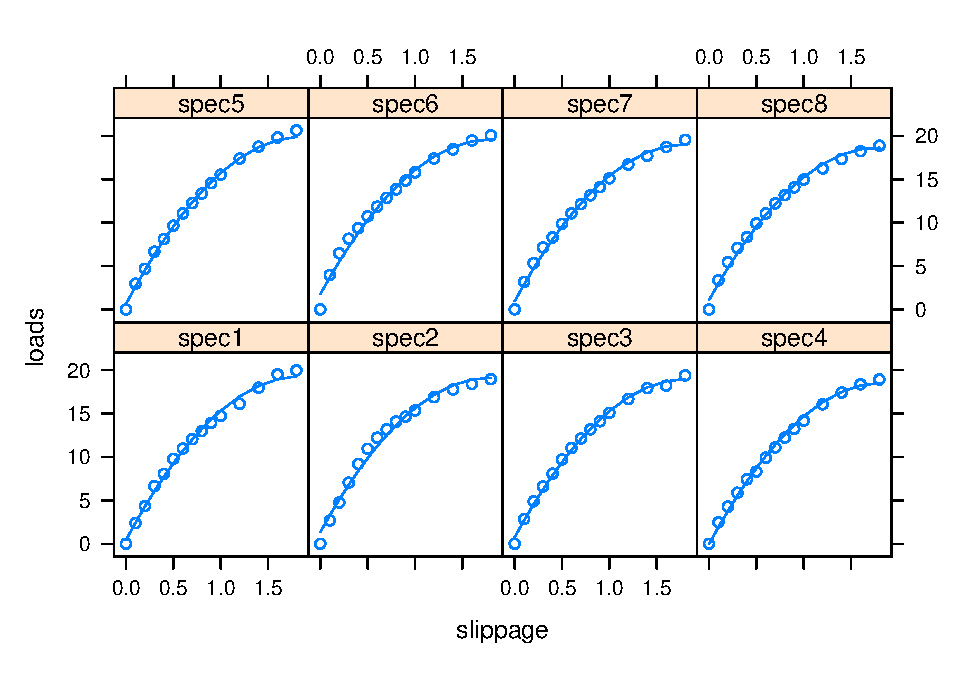
\includegraphics{HUDM6122-Homework_10-Chenguang-Pan_files/figure-latex/unnamed-chunk-3-1.pdf}
Great! All fitted curve goes through the origin!

\hypertarget{ex.-8.2}{%
\subsection{Ex. 8.2}\label{ex.-8.2}}

\emph{Investigate a further model for the glucose challenge data that
allows a random quadratic effect.}

\begin{Shaded}
\begin{Highlighting}[]
\SpecialCharTok{\textgreater{}} \CommentTok{\# import the data}
\ErrorTok{\textgreater{}}\NormalTok{ plasma }\OtherTok{\textless{}{-}} \FunctionTok{plasma}\NormalTok{()}
\SpecialCharTok{\textgreater{}} \FunctionTok{head}\NormalTok{(plasma)}
\NormalTok{       Subject   group time plasma}
\NormalTok{id01}\FloatTok{.1}\NormalTok{    id01 control    }\DecValTok{1}    \FloatTok{4.3}
\NormalTok{id02}\FloatTok{.1}\NormalTok{    id02 control    }\DecValTok{1}    \FloatTok{3.7}
\NormalTok{id03}\FloatTok{.1}\NormalTok{    id03 control    }\DecValTok{1}    \FloatTok{4.0}
\NormalTok{id04}\FloatTok{.1}\NormalTok{    id04 control    }\DecValTok{1}    \FloatTok{3.6}
\NormalTok{id05}\FloatTok{.1}\NormalTok{    id05 control    }\DecValTok{1}    \FloatTok{4.1}
\NormalTok{id06}\FloatTok{.1}\NormalTok{    id06 control    }\DecValTok{1}    \FloatTok{3.8}
\SpecialCharTok{\textgreater{}} \FunctionTok{dim}\NormalTok{(plasma)}
\NormalTok{[}\DecValTok{1}\NormalTok{] }\DecValTok{264}   \DecValTok{4}
\end{Highlighting}
\end{Shaded}

The data looks good.

\begin{Shaded}
\begin{Highlighting}[]
\SpecialCharTok{\textgreater{}} \CommentTok{\# write a new model with random quadratic effect}
\ErrorTok{\textgreater{}}\NormalTok{ plasma.lme3 }\OtherTok{\textless{}{-}} \FunctionTok{lme}\NormalTok{(plasma }\SpecialCharTok{\textasciitilde{}}\NormalTok{ time}\SpecialCharTok{*}\NormalTok{group }\SpecialCharTok{+} \FunctionTok{I}\NormalTok{(time}\SpecialCharTok{\^{}}\DecValTok{2}\NormalTok{),}
\SpecialCharTok{+}                    \AttributeTok{random =} \SpecialCharTok{\textasciitilde{}}\NormalTok{time}\SpecialCharTok{+}\FunctionTok{I}\NormalTok{(time}\SpecialCharTok{\^{}}\DecValTok{2}\NormalTok{)}\SpecialCharTok{|}\NormalTok{Subject,}
\SpecialCharTok{+}                    \AttributeTok{data =}\NormalTok{ plasma, }\AttributeTok{method =} \StringTok{"ML"}\NormalTok{)}
\SpecialCharTok{\textgreater{}} \FunctionTok{summary}\NormalTok{(plasma.lme3)}
\NormalTok{Linear mixed}\SpecialCharTok{{-}}\NormalTok{effects model fit by maximum likelihood}
\NormalTok{  Data}\SpecialCharTok{:}\NormalTok{ plasma }
\NormalTok{       AIC      BIC    logLik}
  \FloatTok{384.9571} \FloatTok{427.8685} \SpecialCharTok{{-}}\FloatTok{180.4786}

\NormalTok{Random effects}\SpecialCharTok{:}
\NormalTok{ Formula}\SpecialCharTok{:} \ErrorTok{\textasciitilde{}}\NormalTok{time }\SpecialCharTok{+} \FunctionTok{I}\NormalTok{(time}\SpecialCharTok{\^{}}\DecValTok{2}\NormalTok{) }\SpecialCharTok{|}\NormalTok{ Subject}
\NormalTok{ Structure}\SpecialCharTok{:}\NormalTok{ General positive}\SpecialCharTok{{-}}\NormalTok{definite, Log}\SpecialCharTok{{-}}\NormalTok{Cholesky parametrization}
\NormalTok{            StdDev     Corr         }
\NormalTok{(Intercept) }\FloatTok{0.79150689}\NormalTok{ (Intr) time  }
\NormalTok{time        }\FloatTok{0.23853208} \SpecialCharTok{{-}}\FloatTok{0.722}       
\FunctionTok{I}\NormalTok{(time}\SpecialCharTok{\^{}}\DecValTok{2}\NormalTok{)   }\FloatTok{0.02225533}  \FloatTok{0.599} \SpecialCharTok{{-}}\FloatTok{0.951}
\NormalTok{Residual    }\FloatTok{0.36633783}              

\NormalTok{Fixed effects}\SpecialCharTok{:}\NormalTok{  plasma }\SpecialCharTok{\textasciitilde{}}\NormalTok{ time }\SpecialCharTok{*}\NormalTok{ group }\SpecialCharTok{+} \FunctionTok{I}\NormalTok{(time}\SpecialCharTok{\^{}}\DecValTok{2}\NormalTok{) }
\NormalTok{                    Value  Std.Error  DF    t}\SpecialCharTok{{-}}\NormalTok{value p}\SpecialCharTok{{-}}\NormalTok{value}
\NormalTok{(Intercept)      }\FloatTok{4.631515} \FloatTok{0.19331352} \DecValTok{228}  \FloatTok{23.958566}   \FloatTok{0e+00}
\NormalTok{time            }\SpecialCharTok{{-}}\FloatTok{0.753964} \FloatTok{0.06354367} \DecValTok{228} \SpecialCharTok{{-}}\FloatTok{11.865284}   \FloatTok{0e+00}
\NormalTok{groupobese       }\FloatTok{1.067254} \FloatTok{0.25322087}  \DecValTok{31}   \FloatTok{4.214716}   \FloatTok{2e{-}04}
\FunctionTok{I}\NormalTok{(time}\SpecialCharTok{\^{}}\DecValTok{2}\NormalTok{)        }\FloatTok{0.084668} \FloatTok{0.00632243} \DecValTok{228}  \FloatTok{13.391706}   \FloatTok{0e+00}
\NormalTok{time}\SpecialCharTok{:}\NormalTok{groupobese }\SpecialCharTok{{-}}\FloatTok{0.125195} \FloatTok{0.03434255} \DecValTok{228}  \SpecialCharTok{{-}}\FloatTok{3.645471}   \FloatTok{3e{-}04}
\NormalTok{ Correlation}\SpecialCharTok{:} 
\NormalTok{                (Intr) time   gropbs }\FunctionTok{I}\NormalTok{(t}\SpecialCharTok{\^{}}\DecValTok{2}\NormalTok{)}
\NormalTok{time            }\SpecialCharTok{{-}}\FloatTok{0.724}                     
\NormalTok{groupobese      }\SpecialCharTok{{-}}\FloatTok{0.516}  \FloatTok{0.144}              
\FunctionTok{I}\NormalTok{(time}\SpecialCharTok{\^{}}\DecValTok{2}\NormalTok{)        }\FloatTok{0.569} \SpecialCharTok{{-}}\FloatTok{0.941}  \FloatTok{0.000}       
\NormalTok{time}\SpecialCharTok{:}\NormalTok{groupobese  }\FloatTok{0.350} \SpecialCharTok{{-}}\FloatTok{0.213} \SpecialCharTok{{-}}\FloatTok{0.678}  \FloatTok{0.000}

\NormalTok{Standardized Within}\SpecialCharTok{{-}}\NormalTok{Group Residuals}\SpecialCharTok{:}
\NormalTok{         Min           Q1          Med           Q3          Max }
\SpecialCharTok{{-}}\FloatTok{2.877281204} \SpecialCharTok{{-}}\FloatTok{0.544442854}  \FloatTok{0.002749287}  \FloatTok{0.560328140}  \FloatTok{2.929399256} 

\NormalTok{Number of Observations}\SpecialCharTok{:} \DecValTok{264}
\NormalTok{Number of Groups}\SpecialCharTok{:} \DecValTok{33} 
\end{Highlighting}
\end{Shaded}

The model looks good. Next, use Likelihood ratio test to compare the
model fit.

\begin{Shaded}
\begin{Highlighting}[]
\SpecialCharTok{\textgreater{}}\NormalTok{ plasma.lme2 }\OtherTok{\textless{}{-}} \FunctionTok{lme}\NormalTok{(plasma }\SpecialCharTok{\textasciitilde{}}\NormalTok{ time}\SpecialCharTok{*}\NormalTok{group }\SpecialCharTok{+} \FunctionTok{I}\NormalTok{(time}\SpecialCharTok{\^{}}\DecValTok{2}\NormalTok{),}
\SpecialCharTok{+}                    \AttributeTok{random =} \SpecialCharTok{\textasciitilde{}}\NormalTok{time}\SpecialCharTok{|}\NormalTok{Subject,}
\SpecialCharTok{+}                    \AttributeTok{data =}\NormalTok{ plasma, }\AttributeTok{method =} \StringTok{"ML"}\NormalTok{)}
\SpecialCharTok{\textgreater{}} \FunctionTok{anova}\NormalTok{(plasma.lme2,plasma.lme3)}
\NormalTok{            Model df      AIC      BIC    logLik   Test  L.Ratio p}\SpecialCharTok{{-}}\NormalTok{value}
\NormalTok{plasma.lme2     }\DecValTok{1}  \DecValTok{9} \FloatTok{383.3149} \FloatTok{415.4984} \SpecialCharTok{{-}}\FloatTok{182.6575}                        
\NormalTok{plasma.lme3     }\DecValTok{2} \DecValTok{12} \FloatTok{384.9571} \FloatTok{427.8685} \SpecialCharTok{{-}}\FloatTok{180.4786} \DecValTok{1}\NormalTok{ vs }\DecValTok{2} \FloatTok{4.357781}  \FloatTok{0.2253}
\end{Highlighting}
\end{Shaded}

Note, the p-value associated with the likelihood ratio test is .2253,
indicating that the random quadratic effect is not better than the
nested model. Therefore, I prefer not to add the random quadratic effect
into the model.

\hypertarget{ex.-8.3}{%
\subsection{Ex. 8.3}\label{ex.-8.3}}

\emph{Fit an independence model to the Beat the Blues data, and compare
the estimated treatment effect confidence interval with that from the
random intercept model described in the text.}

\begin{Shaded}
\begin{Highlighting}[]
\SpecialCharTok{\textgreater{}} \CommentTok{\# import the data}
\ErrorTok{\textgreater{}} \FunctionTok{data}\NormalTok{(}\StringTok{"BtheB"}\NormalTok{, }\AttributeTok{package =} \StringTok{"HSAUR2"}\NormalTok{)}
\SpecialCharTok{\textgreater{}}\NormalTok{ BtheB}\SpecialCharTok{$}\NormalTok{subject }\OtherTok{\textless{}{-}} \FunctionTok{factor}\NormalTok{(}\FunctionTok{rownames}\NormalTok{(BtheB))}
\SpecialCharTok{\textgreater{}}\NormalTok{ nobs }\OtherTok{\textless{}{-}} \FunctionTok{nrow}\NormalTok{(BtheB)}
\SpecialCharTok{\textgreater{}}\NormalTok{ BtheB\_long }\OtherTok{\textless{}{-}} \FunctionTok{reshape}\NormalTok{(BtheB, }\AttributeTok{idvar =} \StringTok{"subject"}\NormalTok{,}
\SpecialCharTok{+}     \AttributeTok{varying =} \FunctionTok{c}\NormalTok{(}\StringTok{"bdi.2m"}\NormalTok{, }\StringTok{"bdi.3m"}\NormalTok{, }\StringTok{"bdi.5m"}\NormalTok{, }\StringTok{"bdi.8m"}\NormalTok{),}
\SpecialCharTok{+}     \AttributeTok{direction =} \StringTok{"long"}\NormalTok{)}
\SpecialCharTok{\textgreater{}}\NormalTok{ BtheB\_long}\SpecialCharTok{$}\NormalTok{time }\OtherTok{\textless{}{-}} \FunctionTok{rep}\NormalTok{(}\FunctionTok{c}\NormalTok{(}\DecValTok{2}\NormalTok{, }\DecValTok{3}\NormalTok{, }\DecValTok{5}\NormalTok{, }\DecValTok{8}\NormalTok{), }\FunctionTok{rep}\NormalTok{(nobs, }\DecValTok{4}\NormalTok{))}
\SpecialCharTok{\textgreater{}} \FunctionTok{head}\NormalTok{(BtheB\_long)}
\NormalTok{     drug length treatment bdi.pre subject time bdi}
\FloatTok{1.2}\NormalTok{m   No    }\SpecialCharTok{\textgreater{}}\NormalTok{6m       TAU      }\DecValTok{29}       \DecValTok{1}    \DecValTok{2}   \DecValTok{2}
\FloatTok{2.2}\NormalTok{m  Yes    }\SpecialCharTok{\textgreater{}}\NormalTok{6m     BtheB      }\DecValTok{32}       \DecValTok{2}    \DecValTok{2}  \DecValTok{16}
\FloatTok{3.2}\NormalTok{m  Yes    }\SpecialCharTok{\textless{}}\NormalTok{6m       TAU      }\DecValTok{25}       \DecValTok{3}    \DecValTok{2}  \DecValTok{20}
\FloatTok{4.2}\NormalTok{m   No    }\SpecialCharTok{\textgreater{}}\NormalTok{6m     BtheB      }\DecValTok{21}       \DecValTok{4}    \DecValTok{2}  \DecValTok{17}
\FloatTok{5.2}\NormalTok{m  Yes    }\SpecialCharTok{\textgreater{}}\NormalTok{6m     BtheB      }\DecValTok{26}       \DecValTok{5}    \DecValTok{2}  \DecValTok{23}
\FloatTok{6.2}\NormalTok{m  Yes    }\SpecialCharTok{\textless{}}\NormalTok{6m     BtheB       }\DecValTok{7}       \DecValTok{6}    \DecValTok{2}   \DecValTok{0}
\SpecialCharTok{\textgreater{}} \FunctionTok{dim}\NormalTok{(BtheB\_long)}
\NormalTok{[}\DecValTok{1}\NormalTok{] }\DecValTok{400}   \DecValTok{7}
\end{Highlighting}
\end{Shaded}

The data looks good. Next, fit an independence model. In an independence
model, the observations at each time point are assumed to be independent
of each other, meaning that there is no correlation between them.

\begin{Shaded}
\begin{Highlighting}[]
\SpecialCharTok{\textgreater{}}\NormalTok{ BtheB\_lme3 }\OtherTok{\textless{}{-}} \FunctionTok{lm}\NormalTok{(bdi }\SpecialCharTok{\textasciitilde{}}\NormalTok{ bdi.pre }\SpecialCharTok{+}\NormalTok{ time }\SpecialCharTok{+}\NormalTok{ treatment}\SpecialCharTok{+}\NormalTok{ drug}\SpecialCharTok{+}\NormalTok{ length }\SpecialCharTok{+}\NormalTok{subject, }
\SpecialCharTok{+}                  \AttributeTok{data =}\NormalTok{ BtheB\_long, }\AttributeTok{na.action =}\NormalTok{ na.omit)}
\SpecialCharTok{\textgreater{}} \FunctionTok{summary}\NormalTok{(BtheB\_lme3)}\SpecialCharTok{$}\NormalTok{coefficients[}\StringTok{"treatmentBtheB"}\NormalTok{, }\FunctionTok{c}\NormalTok{(}\StringTok{"Estimate"}\NormalTok{,}\StringTok{"Std. Error"}\NormalTok{, }
\SpecialCharTok{+}                                                      \StringTok{"t value"}\NormalTok{, }\StringTok{"Pr(\textgreater{}|t|)"}\NormalTok{)]}
\NormalTok{   Estimate  Std. Error     t value    }\FunctionTok{Pr}\NormalTok{(}\SpecialCharTok{\textgreater{}}\ErrorTok{|}\NormalTok{t}\SpecialCharTok{|}\NormalTok{) }
\SpecialCharTok{{-}}\FloatTok{17.1935329}  \FloatTok{11.7573196}  \SpecialCharTok{{-}}\FloatTok{1.4623684}   \FloatTok{0.1453649} 
\end{Highlighting}
\end{Shaded}

From the result, one can have the 95\% confidence interval(CI) is
\(-17.19 \pm 1.96\times11.75= (-40.24, 5.86)\). This treatment effect is
not statistically significant. The 95\% CI from the random intercept
model is \(-2.315 \pm 1.96\times1.72= (-5.69, 1.06)\)

\hypertarget{ex.-8.4}{%
\subsection{Ex. 8.4}\label{ex.-8.4}}

\emph{Construct a plot of the mean profiles of the two treatment groups
in the Beat the Blues study showing also the predicted mean profiles
under the model used in the chapter. Repeat the exercise with a model
that includes only a time effect.}

\begin{Shaded}
\begin{Highlighting}[]
\SpecialCharTok{\textgreater{}} \FunctionTok{library}\NormalTok{(ggplot2)}
\SpecialCharTok{\textgreater{}}\NormalTok{ treatmentlabels }\OtherTok{\textless{}{-}}\FunctionTok{c}\NormalTok{(}\StringTok{\textquotesingle{}TAU\textquotesingle{}}\OtherTok{=}\StringTok{\textquotesingle{}Treatment As Usuaul\textquotesingle{}}\NormalTok{, }\StringTok{\textquotesingle{}BtheB\textquotesingle{}}\OtherTok{=}\StringTok{\textquotesingle{}Beat The Blues\textquotesingle{}}\NormalTok{)}
\SpecialCharTok{\textgreater{}} \FunctionTok{ggplot}\NormalTok{(BtheB\_long, }\FunctionTok{aes}\NormalTok{(time, bdi)) }\SpecialCharTok{+} 
\SpecialCharTok{+}   \FunctionTok{stat\_boxplot}\NormalTok{(}\AttributeTok{geom=}\StringTok{\textquotesingle{}errorbar\textquotesingle{}}\NormalTok{, }\AttributeTok{linetype=}\DecValTok{1}\NormalTok{, }\AttributeTok{width=}\FloatTok{0.5}\NormalTok{) }\SpecialCharTok{+} 
\SpecialCharTok{+}   \FunctionTok{geom\_boxplot}\NormalTok{( }\FunctionTok{aes}\NormalTok{(time, bdi),}\AttributeTok{outlier.shape=}\DecValTok{1}\NormalTok{) }\SpecialCharTok{+} 
\SpecialCharTok{+}   \FunctionTok{facet\_grid}\NormalTok{(}\SpecialCharTok{\textasciitilde{}}\NormalTok{treatment, }\AttributeTok{labeller =} \FunctionTok{as\_labeller}\NormalTok{(treatmentlabels)) }\SpecialCharTok{+}  
\SpecialCharTok{+}   \FunctionTok{stat\_summary}\NormalTok{(}\AttributeTok{fun.y=}\NormalTok{mean, }\AttributeTok{geom=}\StringTok{\textquotesingle{}point\textquotesingle{}}\NormalTok{, }\AttributeTok{size=}\DecValTok{2}\NormalTok{) }\SpecialCharTok{+} 
\SpecialCharTok{+}   \FunctionTok{stat\_summary}\NormalTok{(}\AttributeTok{fun.data=}\NormalTok{mean\_se, }\AttributeTok{geom=}\StringTok{\textquotesingle{}errorbar\textquotesingle{}}\NormalTok{) }\SpecialCharTok{+} 
\SpecialCharTok{+}   \FunctionTok{labs}\NormalTok{(}\AttributeTok{title=}\StringTok{\textquotesingle{}DBI vs Time For Each Treatment Group With Error bars\textquotesingle{}}\NormalTok{, }
\SpecialCharTok{+}        \AttributeTok{x=}\StringTok{\textquotesingle{}Time (Months)\textquotesingle{}}\NormalTok{,}\AttributeTok{y=}\StringTok{\textquotesingle{}BDI\textquotesingle{}}\NormalTok{)}
\end{Highlighting}
\end{Shaded}

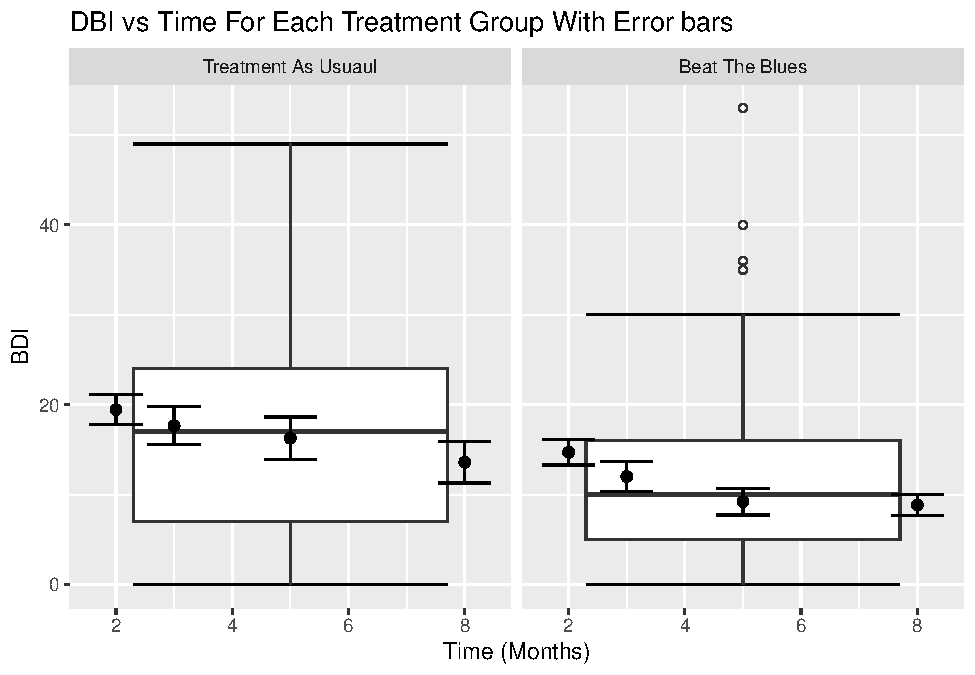
\includegraphics{HUDM6122-Homework_10-Chenguang-Pan_files/figure-latex/unnamed-chunk-9-1.pdf}

\hypertarget{ex.-8.5}{%
\subsection{Ex. 8.5}\label{ex.-8.5}}

\emph{Investigate whether there is any evidence of an interaction
between treatment and time for the Beat the Blues data.}

Reference Note:\\
The following solution refers to the answers on
\href{https://rstudio-pubs-static.s3.amazonaws.com/529736_55aeb8cb60a44adf948c1457e6a00262.html}{this
webpage}. Please click the hyperlink for more detail.

\begin{Shaded}
\begin{Highlighting}[]
\SpecialCharTok{\textgreater{}} \FunctionTok{library}\NormalTok{(}\StringTok{"HSAUR3"}\NormalTok{)}
\SpecialCharTok{\textgreater{}} \FunctionTok{library}\NormalTok{(}\StringTok{"ggplot2"}\NormalTok{)}
\SpecialCharTok{\textgreater{}} \FunctionTok{library}\NormalTok{(}\StringTok{"lme4"}\NormalTok{)}
\SpecialCharTok{\textgreater{}} \FunctionTok{layout}\NormalTok{(}\FunctionTok{matrix}\NormalTok{(}\DecValTok{1}\SpecialCharTok{:}\DecValTok{2}\NormalTok{, }\AttributeTok{nrow=}\DecValTok{1}\NormalTok{))}
\SpecialCharTok{\textgreater{}}\NormalTok{ ylim }\OtherTok{\textless{}{-}} \FunctionTok{range}\NormalTok{(BtheB[,}\FunctionTok{grep}\NormalTok{(}\StringTok{\textquotesingle{}bdi\textquotesingle{}}\NormalTok{, }\FunctionTok{names}\NormalTok{(BtheB))],}
\SpecialCharTok{+}               \AttributeTok{na.rm=}\ConstantTok{TRUE}\NormalTok{)}
\SpecialCharTok{\textgreater{}} 
\ErrorTok{\textgreater{}} 
\ErrorTok{\textgreater{}} \CommentTok{\#subsetting the data for treatment as usual group}
\ErrorTok{\textgreater{}}\NormalTok{ tau }\OtherTok{\textless{}{-}} \FunctionTok{subset}\NormalTok{(BtheB, treatment}\SpecialCharTok{==}\StringTok{\textquotesingle{}TAU\textquotesingle{}}\NormalTok{)[,}\FunctionTok{grep}\NormalTok{(}\StringTok{\textquotesingle{}bdi\textquotesingle{}}\NormalTok{, }\FunctionTok{names}\NormalTok{(BtheB))]}
\SpecialCharTok{\textgreater{}} \CommentTok{\#developing box plots for each time interval for the treatment as usual group based on BDI values}
\ErrorTok{\textgreater{}} \FunctionTok{boxplot}\NormalTok{(tau, }\AttributeTok{main=}\StringTok{\textquotesingle{}Treatment As Usual\textquotesingle{}}\NormalTok{,}\AttributeTok{xlab=}\StringTok{\textquotesingle{}Time (Months)\textquotesingle{}}\NormalTok{, }\AttributeTok{ylab=}\StringTok{\textquotesingle{}BDI\textquotesingle{}}\NormalTok{, }\AttributeTok{ylim=}\NormalTok{ylim, }
\SpecialCharTok{+} \AttributeTok{names=}\FunctionTok{c}\NormalTok{(}\DecValTok{0}\NormalTok{,}\DecValTok{2}\NormalTok{,}\DecValTok{3}\NormalTok{,}\DecValTok{5}\NormalTok{,}\DecValTok{8}\NormalTok{))}
\SpecialCharTok{\textgreater{}} 
\ErrorTok{\textgreater{}} \CommentTok{\#subseting the data for BtheB group}
\ErrorTok{\textgreater{}}\NormalTok{ btb }\OtherTok{\textless{}{-}} \FunctionTok{subset}\NormalTok{(BtheB, treatment}\SpecialCharTok{==}\StringTok{\textquotesingle{}BtheB\textquotesingle{}}\NormalTok{)[,}\FunctionTok{grep}\NormalTok{(}\StringTok{\textquotesingle{}bdi\textquotesingle{}}\NormalTok{, }\FunctionTok{names}\NormalTok{(BtheB))]}
\SpecialCharTok{\textgreater{}} \CommentTok{\#developing box plots for each time interval for the treatment as usual group based on BDI values}
\ErrorTok{\textgreater{}} \FunctionTok{boxplot}\NormalTok{(btb, }\AttributeTok{main=}\StringTok{\textquotesingle{}Beat The Blues\textquotesingle{}}\NormalTok{, }\AttributeTok{xlab=}\StringTok{\textquotesingle{}Time (Months)\textquotesingle{}}\NormalTok{, }\AttributeTok{ylab=}\StringTok{\textquotesingle{}BDI\textquotesingle{}}\NormalTok{, }\AttributeTok{ylim=}\NormalTok{ylim, }\AttributeTok{names=}\FunctionTok{c}\NormalTok{(}\DecValTok{0}\NormalTok{,}\DecValTok{2}\NormalTok{,}\DecValTok{3}\NormalTok{,}\DecValTok{5}\NormalTok{,}\DecValTok{8}\NormalTok{))}
\end{Highlighting}
\end{Shaded}

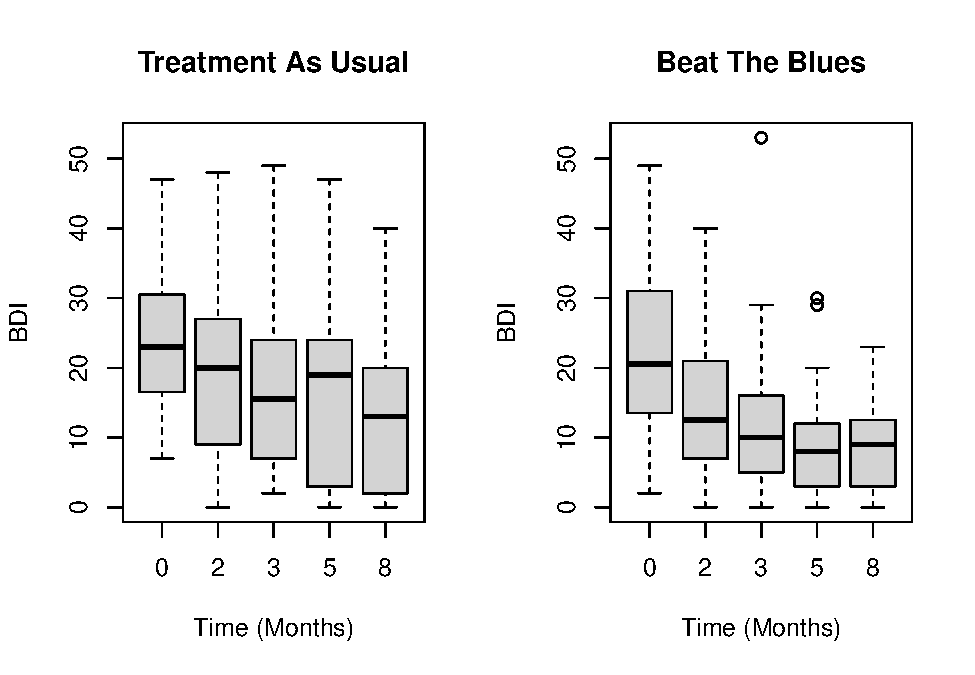
\includegraphics{HUDM6122-Homework_10-Chenguang-Pan_files/figure-latex/unnamed-chunk-10-1.pdf}

\begin{Shaded}
\begin{Highlighting}[]
\SpecialCharTok{\textgreater{}} \CommentTok{\#ggplot can now easily divide the categorical variable (treatment) into its groups TAU vs BtheB}
\ErrorTok{\textgreater{}}\NormalTok{ treatmentlabels }\OtherTok{\textless{}{-}}\FunctionTok{c}\NormalTok{(}\StringTok{\textquotesingle{}TAU\textquotesingle{}}\OtherTok{=}\StringTok{\textquotesingle{}Treatment As Usuaul\textquotesingle{}}\NormalTok{, }\StringTok{\textquotesingle{}BtheB\textquotesingle{}}\OtherTok{=}\StringTok{\textquotesingle{}Beat The Blues\textquotesingle{}}\NormalTok{)}
\SpecialCharTok{\textgreater{}} 
\ErrorTok{\textgreater{}} \FunctionTok{ggplot}\NormalTok{(BtheB\_long, }\FunctionTok{aes}\NormalTok{(time,bdi)) }\SpecialCharTok{+} \FunctionTok{geom\_boxplot}\NormalTok{() }\SpecialCharTok{+} \FunctionTok{facet\_grid}\NormalTok{(}\SpecialCharTok{\textasciitilde{}}\NormalTok{treatment, }\AttributeTok{labeller =} \FunctionTok{as\_labeller}\NormalTok{(treatmentlabels)) }\SpecialCharTok{+} \FunctionTok{labs}\NormalTok{(}\AttributeTok{title=}\StringTok{\textquotesingle{}DBI vs Time For Each Treatment Group\textquotesingle{}}\NormalTok{, }\AttributeTok{x=}\StringTok{\textquotesingle{}Time (Months)\textquotesingle{}}\NormalTok{,}\AttributeTok{y=}\StringTok{\textquotesingle{}BDI\textquotesingle{}}\NormalTok{)}
\end{Highlighting}
\end{Shaded}

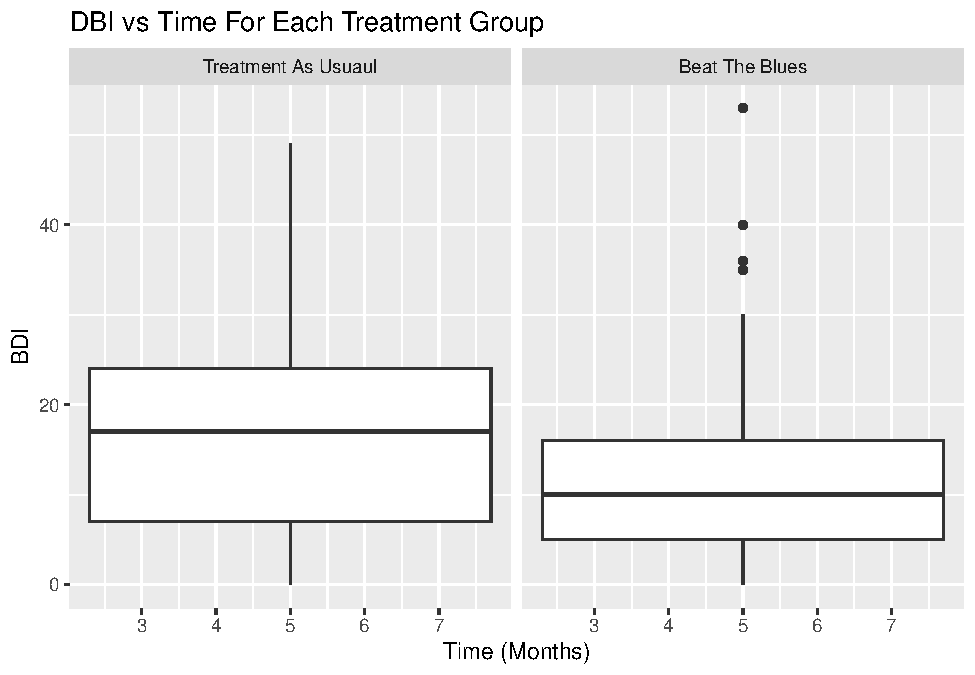
\includegraphics{HUDM6122-Homework_10-Chenguang-Pan_files/figure-latex/unnamed-chunk-11-1.pdf}
Over time, the BDI values show a decreasing trend, while the dispersion
of data in the TAU group appears to be wider than the BtheB group. To
investigate the effect of treatment and its interaction with time, I
will fit both a fixed and mixed model with the same covariates used in
the previous models.

\begin{Shaded}
\begin{Highlighting}[]
\SpecialCharTok{\textgreater{}} \CommentTok{\#Fitting linear model}
\ErrorTok{\textgreater{}}\NormalTok{ btheb\_lm2 }\OtherTok{\textless{}{-}} \FunctionTok{lm}\NormalTok{(bdi }\SpecialCharTok{\textasciitilde{}}\NormalTok{ bdi.pre }\SpecialCharTok{+}\NormalTok{ time }\SpecialCharTok{+}\NormalTok{ drug }\SpecialCharTok{+}\NormalTok{ length }\SpecialCharTok{+}\NormalTok{ treatment }\SpecialCharTok{+}\NormalTok{ subject }\SpecialCharTok{+}\NormalTok{ treatment}\SpecialCharTok{*}\NormalTok{time, }\AttributeTok{data=}\NormalTok{ BtheB\_long)}
\SpecialCharTok{\textgreater{}} 
\ErrorTok{\textgreater{}} \CommentTok{\#Fitting mixed Model}
\ErrorTok{\textgreater{}}\NormalTok{ btheb\_lmer2 }\OtherTok{\textless{}{-}} \FunctionTok{lmer}\NormalTok{(bdi }\SpecialCharTok{\textasciitilde{}}\NormalTok{ bdi.pre }\SpecialCharTok{+}\NormalTok{ time }\SpecialCharTok{+}\NormalTok{ drug }\SpecialCharTok{+}\NormalTok{ length }\SpecialCharTok{+}\NormalTok{ treatment }\SpecialCharTok{+}\NormalTok{ treatment}\SpecialCharTok{*}\NormalTok{time }\SpecialCharTok{+}\NormalTok{ (}\DecValTok{1} \SpecialCharTok{|}\NormalTok{ subject), }\AttributeTok{data=}\NormalTok{BtheB\_long, }\AttributeTok{REML=}\ConstantTok{FALSE}\NormalTok{, }\AttributeTok{na.action=}\NormalTok{na.omit)}
\SpecialCharTok{\textgreater{}} \FunctionTok{anova}\NormalTok{(btheb\_lmer2, btheb\_lm2)}
\NormalTok{Data}\SpecialCharTok{:}\NormalTok{ BtheB\_long}
\NormalTok{Models}\SpecialCharTok{:}
\NormalTok{btheb\_lmer2}\SpecialCharTok{:}\NormalTok{ bdi }\SpecialCharTok{\textasciitilde{}}\NormalTok{ bdi.pre }\SpecialCharTok{+}\NormalTok{ time }\SpecialCharTok{+}\NormalTok{ drug }\SpecialCharTok{+}\NormalTok{ length }\SpecialCharTok{+}\NormalTok{ treatment }\SpecialCharTok{+}\NormalTok{ treatment }\SpecialCharTok{*}\NormalTok{ time }\SpecialCharTok{+}\NormalTok{ (}\DecValTok{1} \SpecialCharTok{|}\NormalTok{ subject)}
\NormalTok{btheb\_lm2}\SpecialCharTok{:}\NormalTok{ bdi }\SpecialCharTok{\textasciitilde{}}\NormalTok{ bdi.pre }\SpecialCharTok{+}\NormalTok{ time }\SpecialCharTok{+}\NormalTok{ drug }\SpecialCharTok{+}\NormalTok{ length }\SpecialCharTok{+}\NormalTok{ treatment }\SpecialCharTok{+}\NormalTok{ subject }\SpecialCharTok{+}\NormalTok{ treatment }\SpecialCharTok{*}\NormalTok{ time}
\NormalTok{            npar    AIC    BIC  logLik deviance  Chisq Df }\FunctionTok{Pr}\NormalTok{(}\SpecialCharTok{\textgreater{}}\NormalTok{Chisq)    }
\NormalTok{btheb\_lmer2    }\DecValTok{9} \FloatTok{1886.7} \FloatTok{1919.4} \SpecialCharTok{{-}}\FloatTok{934.35}   \FloatTok{1868.7}                         
\NormalTok{btheb\_lm2    }\DecValTok{100} \FloatTok{1773.0} \FloatTok{2136.5} \SpecialCharTok{{-}}\FloatTok{786.51}   \FloatTok{1573.0} \FloatTok{295.67} \DecValTok{91}  \SpecialCharTok{\textless{}} \FloatTok{2.2e{-}16} \SpecialCharTok{**}\ErrorTok{*}
\SpecialCharTok{{-}{-}{-}}
\NormalTok{Signif. codes}\SpecialCharTok{:}  \DecValTok{0} \StringTok{\textquotesingle{}***\textquotesingle{}} \FloatTok{0.001} \StringTok{\textquotesingle{}**\textquotesingle{}} \FloatTok{0.01} \StringTok{\textquotesingle{}*\textquotesingle{}} \FloatTok{0.05} \StringTok{\textquotesingle{}.\textquotesingle{}} \FloatTok{0.1} \StringTok{\textquotesingle{} \textquotesingle{}} \DecValTok{1}
\end{Highlighting}
\end{Shaded}

From the results, the fixed model is prefered. Next, checking the
interacion coefficient,

\begin{Shaded}
\begin{Highlighting}[]
\SpecialCharTok{\textgreater{}} \FunctionTok{summary}\NormalTok{(btheb\_lm2)}\SpecialCharTok{$}\NormalTok{coefficients[}\StringTok{"time:treatmentBtheB"}\NormalTok{, }\FunctionTok{c}\NormalTok{(}\StringTok{"Estimate"}\NormalTok{,}\StringTok{"Std. Error"}\NormalTok{, }
\SpecialCharTok{+}                                                      \StringTok{"t value"}\NormalTok{, }\StringTok{"Pr(\textgreater{}|t|)"}\NormalTok{)]}
\NormalTok{  Estimate Std. Error    t value   }\FunctionTok{Pr}\NormalTok{(}\SpecialCharTok{\textgreater{}}\ErrorTok{|}\NormalTok{t}\SpecialCharTok{|}\NormalTok{) }
\FloatTok{0.64357788} \FloatTok{0.29756513} \FloatTok{2.16281351} \FloatTok{0.03186724} 
\end{Highlighting}
\end{Shaded}

The interaction effect is significant in the fixed model.

\end{document}
